\subsection{Basics}
\paragraph{Definition}
It \tB{assumes that $X_{t}$ captures all the relevant information for predicting the future}.
If we assume discrete time steps the \tB{joint distribution} is:
\begin{center}
    \fr{$\prob{\left(X_{t}\right)_{1\leq t\leq T}} = \prob{X_{1}}\prd{t=2}{T}\prob{X_{t}|X_{t-1}}$}
\end{center}
\uB{if the transition function $\prob{X_{t}|X_{t-1}}$ is independent of time then the chain is called
\emph{homogeneous}, \emph{stationary} or \emph{time-invariant}}.\\
This assumption allows us to model an arbitrary of variables using a fixed number of parameters, such
models are called \tB{\textbf{stochastic process}}.

\paragraph{Transition matrix}
\uB{When $X_{t}$ is discrete} the conditional distribution $\prob{X_{t}|X_{t-1}}$ can be written as 
$K\times K$ matrix known as \tB{\textbf{transition matrix} $\bm{A}$, where $A_{ij} = \prob{X_{t}=j|
X_{t-1}=i}$ being the probability of going from state $i$ to $j$}. Each row of the matrix sums to one
\tB{$\Sigma_{j}A_{ij}=1$} so it is called \emph{stochastic matrix}.
\begin{figure}[H]
    \begin{center}
        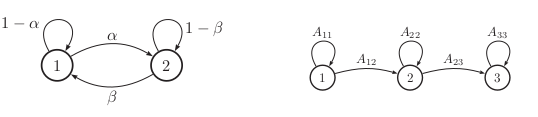
\includegraphics[width=.5\textwidth]{./chapters/2_statistics/07_hidden_markov_models/1_images/1_state_transition_diagrams.png}
    \end{center}
    \caption{State transition diagrams for, 2-state chain and 3-state chain.}
    \label{fig:1_state_transition_diagrams}
\end{figure}

\paragraph{Application}
\begin{itemize}
    \item Sentence completion
    \item Data compression
    \item Text classification
    \item Automatic essay writing
\end{itemize}


\subsection{Basics}
\paragraph{Definition}
It consists of a discrete-time discrete-state Markov chain, with hidden states $z_{t}\in\{k\}_{1\leq
k\leq K}$.\\
The corresponding joint distribution has the form:
$\prob{\left(\bm{z}_{t}\right)_{1\leq t\leq T}, \left(\bm{x}_{t}\right)_{1\leq t\leq T}} = 
\prob{\left(\bm{z}_{t}\right)_{1\leq t\leq T}}
\prob{\left(\bm{z}_{t}\right)_{1\leq t\leq T}| \left(\bm{x}_{t}\right)_{1\leq t\leq T}}  =
\left[\prob{z_{1}}\prd{t=2}{T}\prob{z_{t}|z_{t-1}}\right] = \prd{t=2}{T}\prob{\bm{x}_{t}|z_{t}}$
\begin{itemize}
    \item \emph{discrete}: $\prob{\bm{x}_{t}=l|z_{t}=k,\bm{\theta}} = \text{\emph{Beta}}(k,l)$
    \item \emph{discrete}: $\prob{\bm{x}_{t}|z_{t}=k,\bm{\theta}} = \mathcal{N}(\bm{x}_{t}|
        \bm{\mu}_{k},\bm{\Sigma}_{k})$
\end{itemize}

